\documentclass[11pt]{beamer}
\usepackage[utf8]{inputenc}
\usepackage[T1]{fontenc}
\usepackage{lmodern}
\usepackage[english]{babel}
\usepackage{booktabs}
\usepackage{fontawesome}
\usetheme{Darmstadt}
\setbeamertemplate{navigation symbols}{}
\setbeamertemplate{footline}{
	\begin{beamercolorbox}[ht=3ex,leftskip=1.4cm,rightskip=.3cm]{author in head/foot}
		\hfill \insertframenumber
		\vspace*{0.07cm}
	\end{beamercolorbox}
} 
\usepackage{url}
\usepackage{hyperref}

% color def
\usepackage{color}
\definecolor{darkred}{rgb}{0.6,0.0,0.0}
\definecolor{darkgreen}{rgb}{0,0.50,0}
\definecolor{lightblue}{rgb}{0.0,0.42,0.91}
\definecolor{orange}{rgb}{0.99,0.48,0.13}
\definecolor{grass}{rgb}{0.18,0.80,0.18}
\definecolor{pink}{rgb}{0.97,0.15,0.45}

\usepackage{listings}
\usepackage{upquote}


\newcommand\Wider[2][3em]{%
\makebox[\linewidth][c]{%
  \begin{minipage}{\dimexpr\textwidth+#1\relax}
  \raggedright#2
  \end{minipage}%
  }%
}

\lstdefinestyle{Python}{
    language=Python,
    morekeywords=[1]{,as,assert,nonlocal,with,yield,self,True,False,None,} % Python builtin
	morekeywords=[2]{,__init__,__add__,__mul__,__div__,__sub__,__call__,__getitem__,__setitem__,__eq__,__ne__,__nonzero__,__rmul__,__radd__,__repr__,__str__,__get__,__truediv__,__pow__,__name__,__future__,__all__,}, % magic methods
	morekeywords=[3]{,object,type,isinstance,copy,deepcopy,zip,enumerate,reversed,list,set,len,dict,tuple,range,xrange,append,execfile,real,imag,reduce,str,repr,}, % common functions
	morekeywords=[4]{,Exception,NameError,IndexError,SyntaxError,TypeError,ValueError,OverflowError,ZeroDivisionError,}, % errors
	morekeywords=[5]{,ode,fsolve,sqrt,exp,sin,cos,arctan,arctan2,arccos,pi, array,norm,solve,dot,arange,isscalar,max,sum,flatten,shape,reshape,find,any,all,abs,plot,linspace,legend,quad,polyval,polyfit,hstack,concatenate,vstack,column_stack,empty,zeros,ones,rand,vander,grid,pcolor,eig,eigs,eigvals,svd,qr,tan,det,logspace,roll,min,mean,cumsum,cumprod,diff,vectorize,lstsq,cla,eye,xlabel,ylabel,squeeze,}, % numpy / math
	%morestring=*[b]{"},
    basicstyle=\ttfamily,
   	backgroundcolor=\color{white},
   	commentstyle=\color{darkgreen}\slshape,
   	keywordstyle=\color{blue}\bfseries\itshape,
   	keywordstyle=[2]\color{blue}\bfseries,
   	keywordstyle=[3]\color{grass},
   	keywordstyle=[4]\color{red},
   	keywordstyle=[5]\color{orange},
   	stringstyle=\color{darkred},
   	emphstyle=\color{pink}\underbar,
    % honek neretako bakarrik die
    %deletekeywords=[2]{next,set},
    %deletekeywords=[3]{next,set},
}

% General Setting of listings
\lstset{
    style=Python,
	tabsize=4,
	aboveskip=1em,
	breaklines=true,
	abovecaptionskip=-6pt,
	captionpos=b,
	escapeinside={\%*}{*)},
	frame=single,
	numbers=left,
	numbersep=8pt,
	numberstyle=\tiny,
    showstringspaces=false,
}

\definecolor{delim}{RGB}{20,105,176}
\definecolor{numb}{RGB}{106, 109, 32}
\definecolor{string}{rgb}{0.64,0.08,0.08}

\lstdefinelanguage{json}{
    showspaces=false,
    showtabs=false,
    breaklines=true,
    postbreak=\raisebox{0ex}[0ex][0ex]{\ensuremath{\color{gray}\hookrightarrow\space}},
    breakatwhitespace=true,
    basicstyle=\ttfamily\small,
    upquote=true,
    morestring=[b]",
    stringstyle=\color{string},
    literate=
     *{0}{{{\color{numb}0}}}{1}
      {1}{{{\color{numb}1}}}{1}
      {2}{{{\color{numb}2}}}{1}
      {3}{{{\color{numb}3}}}{1}
      {4}{{{\color{numb}4}}}{1}
      {5}{{{\color{numb}5}}}{1}
      {6}{{{\color{numb}6}}}{1}
      {7}{{{\color{numb}7}}}{1}
      {8}{{{\color{numb}8}}}{1}
      {9}{{{\color{numb}9}}}{1}
      {\{}{{{\color{delim}{\{}}}}{1}
      {\}}{{{\color{delim}{\}}}}}{1}
      {[}{{{\color{delim}{[}}}}{1}
      {]}{{{\color{delim}{]}}}}{1},
}

\usepackage{tikz}
\usetikzlibrary{calc,shapes.multipart,chains,arrows,positioning}
\usetikzlibrary {shapes.misc} 
\usetikzlibrary{shadows.blur}
\usetikzlibrary{matrix}
\tikzset{
stack_item/.style={rounded rectangle, rounded rectangle arc length=90,draw, anchor=center, fill=white, minimum width=2cm, minimum height=0.7cm},
bar/.style={rounded rectangle, minimum width=3cm, fill=black, blur shadow={shadow blur steps=5,shadow blur extra rounding=1.3pt}},
message/.style={rectangle, fill=white, color=white, text=black},
bowling_pin/.style={circle, draw, line width=0.6mm, color=red, text=black, minimum width=8mm},
empty/.style={circle, draw, line width=0.6mm, color=white, text=black, minimum width=8mm},
table_cell/.style={rectangle, draw, color=black, text=black, minimum size=12mm}
}

\tikzset{
	squarecross/.style={
		draw, rectangle,minimum size=18pt, fill=orange!80,
		inner sep=0pt, text=black,
		path picture = {
			\draw[-,black]
			(path picture bounding box.north west) --
			(path picture bounding box.south east)
			(path picture bounding box.south west) --
			(path picture bounding box.north east);
		}
	},
	list/.style={
		very thick, rectangle split,
		rectangle split parts=2, draw,
		rectangle split horizontal, minimum size=18pt,
		inner sep=4pt, text=black,
		rectangle split part fill={red!20, blue!20}
	},
	->, start chain, very thick,
	chain_arrow/.style={*->, thick}
}

\usetikzlibrary{arrows.meta}
\tikzset{
    queue element/.style={
        draw,very thin,rounded corners,
        fill=white,
        minimum width=1cm,minimum height=.5cm,
        font=\sffamily\footnotesize
    },
    >={[scale=0.8]Triangle}
}

\author{Data Structures}
\title{\huge{Stacks and Queues}}
\titlegraphic{
\includegraphics[width=3cm]{img/UPNA}}
\date[]{2024-2025}
\subject{Data Structures}
%\subtitle{}
%\logo{}
%\institute{}
%\date{}
%\subject{}
%\setbeamercovered{transparent}
%\setbeamertemplate{navigation symbols}{}

\AtBeginSection[]{
	\begin{frame}[plain]
		\frametitle{}
		\tableofcontents[currentsection, hideothersubsections]
	\end{frame}
}

\begin{document}
\begin{frame}[plain]
	\maketitle
\end{frame}

\begin{frame}
	\tableofcontents
\end{frame}

\section{Abstract Data Types}

\begin{frame}\frametitle{What is an \textit{ADT}}
\begin{itemize}
\item An \textit{Abstract Data Type} (ADT) is a way to model the interaction a user has with the data
\item The structure is defined only conceptually
    \begin{itemize}
    \item Possible values
    \item Operations on the data type and their behaviour
    \end{itemize}
\item An ADT describes the logical form of the data, a \textbf{data structure} is its implementation
\end{itemize}
\end{frame}

\section{\textit{ADTs} implemented on Python}

\begin{frame}\frametitle{Some ADTs are already implemented on Python}
\begin{itemize}
\item Most of the programming languages already implement a few ADTs
\item Python has several in the core libraries:
    \begin{itemize}
    \item Lists
    \item Maps (Dictionaries)
    \item Sets
    \end{itemize}
\item There are more in external libraries
    \begin{itemize}
    \item Queues/Deques
    \item Trees
    \item Graphs
    \end{itemize}
\end{itemize}
\end{frame}

\subsection{Lists}

\begin{frame}\frametitle{The List ADT}
\begin{itemize}
\item The \texttt{List} is one of the most common ADT
\item It stores data points in a given order
    \begin{itemize}
    \item The length of the list is usually dynamic
    \end{itemize}
\item Basic \texttt{List} methods
    \begin{itemize}
    \item Create an empty list
    \item Test if the list is empty
    \item Add an element to the list
    \item Remove an element from the list
    \item Access an element with an index
    \end{itemize}
\end{itemize}
\vspace{0.4cm}
\begin{center}
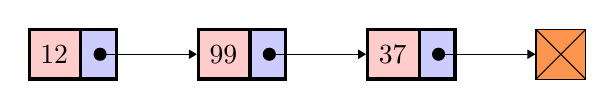
\begin{tikzpicture}
  \node[list,on chain] (A) {12};
  \node[list,on chain] (B) {99};
  \node[list,on chain] (C) {37};
  \node[squarecross]   (D) [right=of C] {};
  \draw[*->] let \p1 = (A.two), \p2 = (A.center) in (\x1,\y2) -- (B);
  \draw[*->] let \p1 = (B.two), \p2 = (B.center) in (\x1,\y2) -- (C);
  \draw[*->] let \p1 = (C.two), \p2 = (C.center) in (\x1,\y2) -- (D);
\end{tikzpicture}
\end{center}
\end{frame}

\begin{frame}\frametitle{Lists in Python}

\Wider{\centering\scriptsize
\begin{tabular}{@{}lll@{}}
\toprule
\textbf{Method} & \textbf{Use} & \textbf{Explanation} \\
\midrule
\texttt{append} & \texttt{a\_list.append(item)} & Adds a new item to the end of a list \\
\texttt{insert} & \texttt{a\_list.insert(i, item)} & Inserts an item at the $i^{th}$ position in a list \\
\texttt{pop} & \texttt{a\_list.pop()} & Removes and returns the last item in a list \\
\texttt{pop} & \texttt{a\_list.pop(i)} & Removes and returns the $i^{th}$ item in a list \\
\texttt{sort} & \texttt{a\_list.sort()} & Modifies a list to be sorted \\
\texttt{reverse} & \texttt{a\_list.reverse()} & Modifies a list to be in reverse order \\
\texttt{\textbf{del}} & \texttt{\textbf{del} a\_list[i]} & Deletes the item in the $i^{th}$ position \\
\texttt{index} & \texttt{a\_list.index(item)} & Returns the index of the first occurrence of item \\
\texttt{count} & \texttt{a\_list.count(item)} & Returns the number of occurrences of item \\
\texttt{remove} & \texttt{a\_list.remove(item)} & Removes the first occurrence of item \\
\bottomrule
\end{tabular}
}
\vspace{0.4cm}
\begin{block}{More information}
\href{https://docs.python.org/3/tutorial/datastructures.html}{\color{blue}\underline{https://docs.python.org/3/tutorial/datastructures.html}}
\end{block}
\end{frame}

\subsection{Maps}

\begin{frame}\frametitle{The Map ADT}
\begin{itemize}
\item A \texttt{Map} is a collection of $<key, value>$ pairs
\item It can be implemented using hash tables, search trees or other structures
\item Basic \texttt{Map} methods:
    \begin{itemize}
    \item Insert a new $<key, value>$ pair
    \item Remove a $<key, value>$ pair
    \item Get a value from a given key
    \end{itemize}
\end{itemize}
\end{frame}

\begin{frame}\frametitle{Maps in Python}
\Wider{\centering\scriptsize
\begin{tabular}{@{}lll@{}}
\toprule
\textbf{Method} & \textbf{Use} & \textbf{Explanation} \\
\midrule
 & \texttt{a\_dict[key] = value} & Set a value for a key \\
 & \texttt{a\_dict[key]} & Returns the value associated with key \\
\texttt{keys} & \texttt{a\_dict.keys()} & Return the keys of the dictionary in a \texttt{dict\_keys} object \\
\texttt{values} & \texttt{a\_dict.values()} & Return the keys of the dictionary in a \texttt{dict\_values} object \\
\texttt{items} & \texttt{a\_list.items} & Return the key-value pairs in a \texttt{dict\_items} object \\
\texttt{get} & \texttt{a\_list.get(key)} & Returns the value associated with \texttt{key}, \texttt{None} otherwise \\
\texttt{get} & \texttt{a\_list.get(key, alt)} & Returns the value associated with \texttt{key}, \texttt{alt} otherwise \\
\bottomrule
\end{tabular}
\normalsize
\vspace{0.4cm}

\begin{block}{More information}
\href{https://docs.python.org/3/tutorial/datastructures.html\#dictionaries}{\color{blue}\underline{https://docs.python.org/3/tutorial/datastructures.html\#dictionaries}}
\end{block}
}
\end{frame}

\section{Stack}

\begin{frame}\frametitle{The Stack ADT}
\begin{itemize}
\item Last in First out (LIFO)
\end{itemize}
\vspace{0.4cm}
\begin{center}
\scalebox{1.5}{
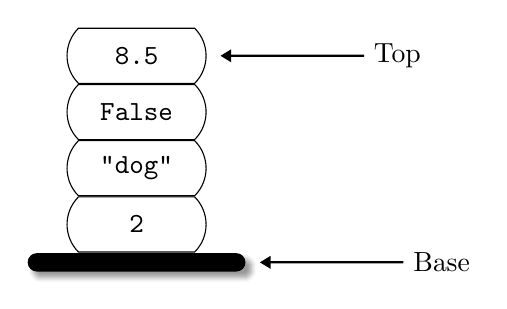
\begin{tikzpicture}
    \node[bar] (base_1) {};
    \node[stack_item] (1_1) [above=0 of base_1] {\texttt{2}};
    \node[stack_item] (1_2) [above=0 of 1_1] {\texttt{"dog"}};
    \node[stack_item] (1_3) [above=0 of 1_2] {\texttt{False}};
    \node[stack_item] (1_4) [above=0 of 1_3] {\texttt{8.5}};
    \node (base) [right=2cm of base_1] {Base};
    \node (text) [right=2cm of 1_4] {Top};
    \draw[->, shorten >=5pt, thick] (base) -- (base_1);
    \draw[->, shorten >=5pt, thick] (text) -- (1_4);
\end{tikzpicture}
}
\end{center}
\end{frame}

\begin{frame}\frametitle{Operating on an Stack}
\begin{itemize}
\item The Stack will have at least two operations
    \begin{description}
    \item[push:] Add a new item at the top of the Stack
    \item[pop:] Remove and return the top element of the Stack
    \end{description}
\item There can be more optional operations
    \begin{description}
    \item[peek:] Return the top element of the Stack without removing it
    \item[is\_empty:] Returns \lstinline|True| if the Stack is empty, \lstinline|False| otherwise
    \item[size:] Returns the number of elements on the Stack
    \end{description}
\end{itemize}
\end{frame}

\begin{frame}\frametitle{The push operation I}
\begin{center}
\scalebox{1.5}{
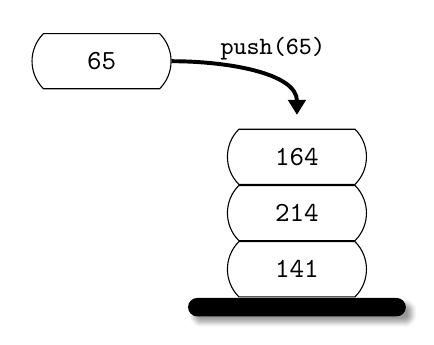
\begin{tikzpicture}
    \node[bar] (base_1) {};
    \node[stack_item] (1_1) [above=0 of base_1] {\texttt{141}};
    \node[stack_item] (1_2) [above=0 of 1_1] {\texttt{214}};
    \node[stack_item] (1_3) [above=0 of 1_2] {\texttt{164}};
    \node[stack_item] (1_4) [above left=0.5 and 1 of 1_3] {\texttt{65}};
    \draw[->, shorten >=5pt, line width=0.5mm] (1_4.east) to [out=0,in=90] (1_3.north) node[midway, above left=3cm and -0.5cm] {\small\texttt{push(65)}};
\end{tikzpicture}
}
\end{center}
\end{frame}

\begin{frame}\frametitle{The push operation II}
\begin{center}
\scalebox{1.5}{
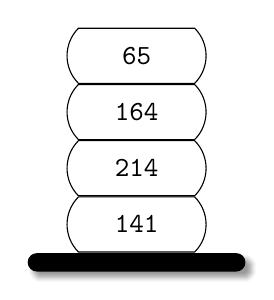
\begin{tikzpicture}
    \node[bar] (base_1) {};
    \node[stack_item] (1_1) [above=0 of base_1] {\texttt{141}};
    \node[stack_item] (1_2) [above=0 of 1_1] {\texttt{214}};
    \node[stack_item] (1_3) [above=0 of 1_2] {\texttt{164}};
    \node[stack_item] (1_4) [above=0 of 1_3] {\texttt{65}};
\end{tikzpicture}
}
\end{center}
\end{frame}

\begin{frame}\frametitle{The pop operation I}
\begin{center}
\scalebox{1.5}{
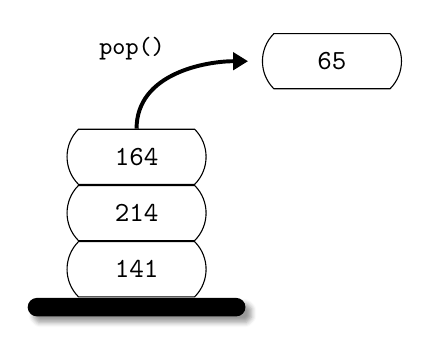
\begin{tikzpicture}
    \node[bar] (base_1) {};
    \node[stack_item] (1_1) [above=0 of base_1] {\texttt{141}};
    \node[stack_item] (1_2) [above=0 of 1_1] {\texttt{214}};
    \node[stack_item] (1_3) [above=0 of 1_2] {\texttt{164}};
    \node[stack_item] (1_4) [above right=0.5 and 1 of 1_3] {\texttt{65}};
    \draw[->, shorten >=5pt, line width=0.5mm] (1_3.north) to [out=90,in=180] (1_4.west) node[midway, above left=3cm and -0.5cm] {\small\texttt{pop()}};
\end{tikzpicture}
}
\end{center}
\end{frame}

\begin{frame}\frametitle{The pop operation II}
\begin{center}
\scalebox{1.5}{
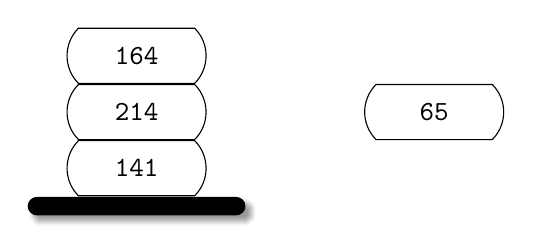
\begin{tikzpicture}
    \node[bar] (base_1) {};
    \node[stack_item] (1_1) [above=0 of base_1] {\texttt{141}};
    \node[stack_item] (1_2) [above=0 of 1_1] {\texttt{214}};
    \node[stack_item] (1_3) [above=0 of 1_2] {\texttt{164}};
    \node[stack_item] (1_4) [right=2 of 1_2] {\texttt{65}};
\end{tikzpicture}
}
\end{center}
\end{frame}

\begin{frame}\frametitle{The peek operation I}
\begin{center}
\scalebox{1.5}{
\begin{tikzpicture}
    \node[bar] (base_1) {};
    \node[stack_item] (1_1) [above=0 of base_1] {\texttt{141}};
    \node[stack_item] (1_2) [above=0 of 1_1] {\texttt{214}};
    \node[stack_item] (1_3) [above=0 of 1_2] {\texttt{164}};
    \node[stack_item] (1_4) [above=0 of 1_3] {\texttt{65}};
    \node (eye) [left=1.5 of 1_4] {\Huge\faEye};
    \draw[->, shorten >=5pt, line width=0.5mm] (eye) to (1_4) node[midway, above left=2.6cm and 1cm] {\small\texttt{peek()}};
\end{tikzpicture}
}
\end{center}
\end{frame}

\begin{frame}\frametitle{The peek operation II}
\begin{center}
\scalebox{1.5}{
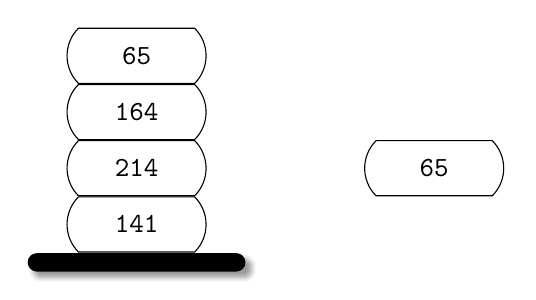
\begin{tikzpicture}
    \node[bar] (base_1) {};
    \node[stack_item] (1_1) [above=0 of base_1] {\texttt{141}};
    \node[stack_item] (1_2) [above=0 of 1_1] {\texttt{214}};
    \node[stack_item] (1_3) [above=0 of 1_2] {\texttt{164}};
    \node[stack_item] (1_4) [above=0 of 1_3] {\texttt{65}};
    \node[stack_item] (1_5) [right=2 of 1_2] {\texttt{65}};
\end{tikzpicture}
}
\end{center}
\end{frame}

\begin{frame}\frametitle{Stack Creation}
\begin{block}{}
\centering\Huge How would you create a Stack using Python?
\end{block}
\end{frame}


\section{Queue}

\begin{frame}\frametitle{The Queue ADT}
\begin{itemize}
\item First in First out (FIFO)
\end{itemize}
\vspace{0.4cm}
\begin{center}
\scalebox{1.5}{
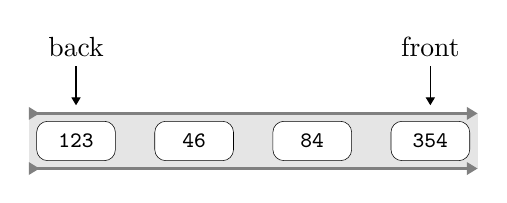
\begin{tikzpicture}
\fill[gray!20] (5.1,.35) rectangle (-.6,-.35);
\draw[gray,thick,>->] (-.6,.35) -- (5.1,.35);
\draw[gray,thick,>->] (-.6,-.35) -- (5.1,-.35);
\foreach \i/\name in {0/123,1/46,2/84,3/354}
    \node[queue element] (elem_\i) at (1.5*\i,0) {\texttt{\name}};
\draw[<-] ([yshift=.2cm]elem_3.north) -- ++ (0,.5) node[above] {front};
\draw[<-] ([yshift=.2cm]elem_0.north) -- ++ (0,.5) node[above] {back};
\end{tikzpicture}
}
\end{center}
\end{frame}

\begin{frame}\frametitle{Operating on a Queue}
\begin{itemize}
\item The Queue will have at least two operations
    \begin{description}
    \item[enqueue:] Add a new item at the back of the Queue
    \item[dequeue:] Remove and return an item from the front of the Queue
    \end{description}
\item As with the Stacks a Queue may have more operations
    \begin{description}
    \item[peek:] Return the front element of the Queue without removing it
    \item[is\_empty:] Returns \lstinline|True| if the Queue is empty, \lstinline|False| otherwise
    \item[size:] Returns the number of elements on the Queue
    \end{description}
\end{itemize}
\end{frame}

\begin{frame}\frametitle{The enqueue operation I}
\begin{center}
\scalebox{1.5}{
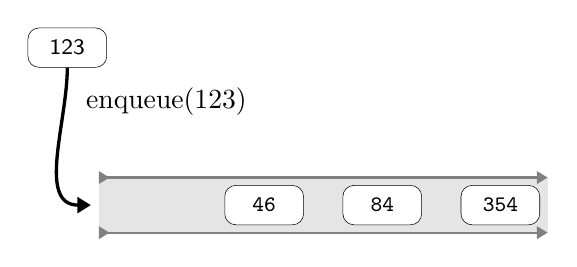
\begin{tikzpicture}
\fill[gray!20] (5.1,.35) rectangle (-.6,-.35);
\draw[gray,thick,>->] (-.6,.35) -- (5.1,.35);
\draw[gray,thick,>->] (-.6,-.35) -- (5.1,-.35);
\foreach \i/\name in {1/46,2/84,3/354}
    \node[queue element] (elem_\i) at (1.5*\i,0) {\texttt{\name}};
\node[queue element] (0) at (-1,2) {123};
\draw[->,very thick] (0.south) to[out=-90,in=180] (-.7,0) node[midway, above right=1 and -0.9] {enqueue(123)};
\end{tikzpicture}
}
\end{center}
\end{frame}

\begin{frame}\frametitle{The enqueue operation II}
\begin{center}
\scalebox{1.5}{
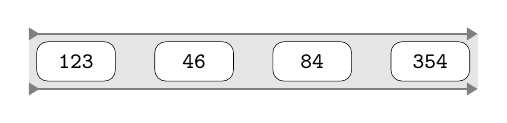
\begin{tikzpicture}
\fill[gray!20] (5.1,.35) rectangle (-.6,-.35);
\draw[gray,thick,>->] (-.6,.35) -- (5.1,.35);
\draw[gray,thick,>->] (-.6,-.35) -- (5.1,-.35);
\foreach \i/\name in {0/123,1/46,2/84,3/354}
    \node[queue element] (elem_\i) at (1.5*\i,0) {\texttt{\name}};
\end{tikzpicture}
}
\end{center}
\end{frame}


\begin{frame}\frametitle{The dequeue operation I}
\begin{center}
\scalebox{1.5}{
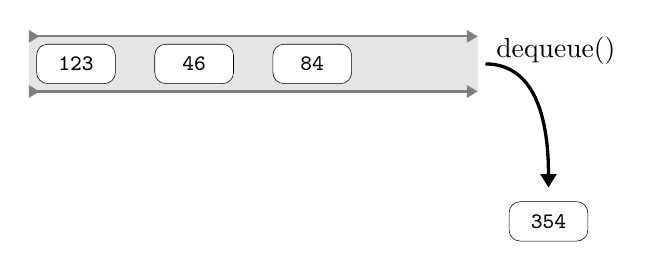
\begin{tikzpicture}
\fill[gray!20] (5.1,.35) rectangle (-.6,-.35);
\draw[gray,thick,>->] (-.6,.35) -- (5.1,.35);
\draw[gray,thick,>->] (-.6,-.35) -- (5.1,-.35);
\foreach \i/\name in {0/123,1/46,2/84}
    \node[queue element] (elem_\i) at (1.5*\i,0) {\texttt{\name}};
\node[queue element] (3) at (6,-2) {\texttt{354}};
\draw[->,very thick, shorten >=5pt] (5.2,0) to[out=0,in=90] (3.north) node[above right=1.6 and -0.8] {dequeue()};
\end{tikzpicture}
}
\end{center}
\end{frame}


\begin{frame}\frametitle{The dequeue operation II}
\begin{center}
\scalebox{1.5}{
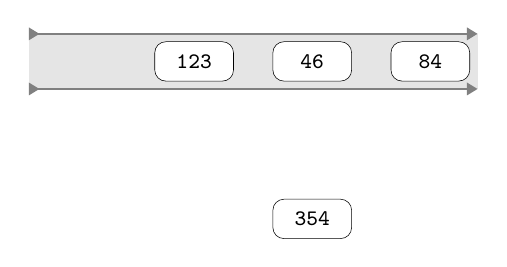
\begin{tikzpicture}
\fill[gray!20] (5.1,.35) rectangle (-.6,-.35);
\draw[gray,thick,>->] (-.6,.35) -- (5.1,.35);
\draw[gray,thick,>->] (-.6,-.35) -- (5.1,-.35);
\foreach \i/\name in {1/123,2/46,3/84}
    \node[queue element] (elem_\i) at (1.5*\i,0) {\texttt{\name}};
\node[queue element] (4) at (3,-2) {\texttt{354}};
\end{tikzpicture}
}
\end{center}
\end{frame}

\begin{frame}\frametitle{The peek operation I}
\begin{center}
\scalebox{1.5}{
\begin{tikzpicture}
\fill[gray!20] (5.1,.35) rectangle (-.6,-.35);
\draw[gray,thick,>->] (-.6,.35) -- (5.1,.35);
\draw[gray,thick,>->] (-.6,-.35) -- (5.1,-.35);
\foreach \i/\name in {0/123,1/46,2/84,3/354}
    \node[queue element] (elem_\i) at (1.5*\i,0) {\texttt{\name}};
\node (eye) [above=1.5 of elem_3] {\Huge\faEye};
\draw[->, shorten >=5pt, line width=0.5mm] (eye) to (elem_3) node[above right=1cm and 0cm] {\small\texttt{peek()}};
\end{tikzpicture}
}
\end{center}
\end{frame}

\begin{frame}\frametitle{The peek operation II}
\begin{center}
\scalebox{1.5}{
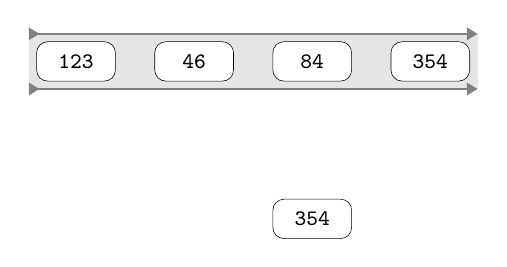
\begin{tikzpicture}
\fill[gray!20] (5.1,.35) rectangle (-.6,-.35);
\draw[gray,thick,>->] (-.6,.35) -- (5.1,.35);
\draw[gray,thick,>->] (-.6,-.35) -- (5.1,-.35);
\foreach \i/\name in {0/123,1/46,2/84,3/354}
    \node[queue element] (elem_\i) at (1.5*\i,0) {\texttt{\name}};
\node[queue element] (4) at (3,-2) {\texttt{354}};
\end{tikzpicture}
}
\end{center}
\end{frame}

\begin{frame}\frametitle{Queue Creation}
\begin{block}{}
\centering\Huge How would you create a Queue using Python?
\end{block}
\end{frame}

%\section{JSON}
%
%\begin{frame}\frametitle{What is JSON}
%\begin{itemize}
%\item Oringinated from JavaScript $\rightarrow$ JavaScript Object Notation
%    \begin{itemize}
%    \item Language-independent
%    \item Many modern languages have support to generate or parse it
%    \end{itemize}
%\item A standard for data interchange using human-readable text
%    \begin{itemize}
%    \item An alternative to XML
%    \end{itemize}
%\item Data is stored in $<attribute,value>$ pairs
%    \begin{itemize}
%    \item Similar to a dictionary in Python
%    \end{itemize}
%\end{itemize}
%\end{frame}
%
%
%\begin{frame}[fragile]\frametitle{JSON example}
%\begin{lstlisting}[basicstyle=\ttfamily\tiny,numberstyle=\tiny]
%{
%  "first_name": "John",
%  "last_name": "Smith",
%  "is_alive": true,
%  "age": 27,
%  "address": {
%    "street_address": "21 2nd Street",
%    "city": "New York",
%    "state": "NY",
%    "postal_code": "10021-3100"
%  },
%  "phone_numbers": [
%    {
%      "type": "home",
%      "number": "212 555-1234"
%    },
%    {
%      "type": "office",
%      "number": "646 555-4567"
%    }
%  ]
%}
%\end{lstlisting}
%\end{frame}
%
%\begin{frame}\frametitle{JSON Data Types}
%\begin{description}
%\item[Object:] The $<key, value>$ pairs, similar to a \lstinline|dict|
%\item[Number:] A number, similar to a \lstinline|float|
%\item[String:] A sequence of characters delimited by double quotes
%\item[Boolean:] A \lstinline|true| or \lstinline|false| value
%\item[Array:] A ordered list of elements, similar to \lstinline|list|
%\item[null:] An empty value, similar to \lstinline|None|
%\end{description}
%\end{frame}
%
%\begin{frame}\frametitle{Webpages to Play with JSON}
%\begin{itemize}
%\setlength\itemsep{0.4cm}
%\item \href{http://www.json.org/json-en.html}{\color{blue}\underline{http://www.json.org/json-en.html}}
%\item \href{https://codebeautify.org/jsonviewer}{\color{blue}\underline{https://codebeautify.org/jsonviewer}}
%\item \href{http://jsonviewer.stack.hu/}{\color{blue}\underline{http://jsonviewer.stack.hu/}}
%\end{itemize}
%\end{frame}



\end{document}